\chapter{Future Work}\label{chapter:future_work}

%Building on the progress made so far, additional energy profiles must be created to develop a robust energy inference function. This task involves collecting profiles from different machines and gathering enough data to effectively train the machine learning model. The static analysis tool will be implemented and used to provide important code, specifically, certain features that will feed into the model.

%After that the efforts will be on developing the actual energy inference function. This task is expected to be the most time-consuming, as it is crucial to the tool functioning. It is most likely that this task overlaps the energy profiling task as more profiles might need to be collected. The task will start by implementing the ML algorithms described in \ref{sec:background_machine_learning}, test their accuracy and improving it by tuning the energy profiles for many possible cases.

%When the function is completed, it will be tested against other tools to ensure its quality. The extension will then be built and tested in IDEs.
%While developing the function and the extension, the writing of the thesis will also be done in parallel documenting every information.

%\begin{figure*}%[h]
%  \centering
%  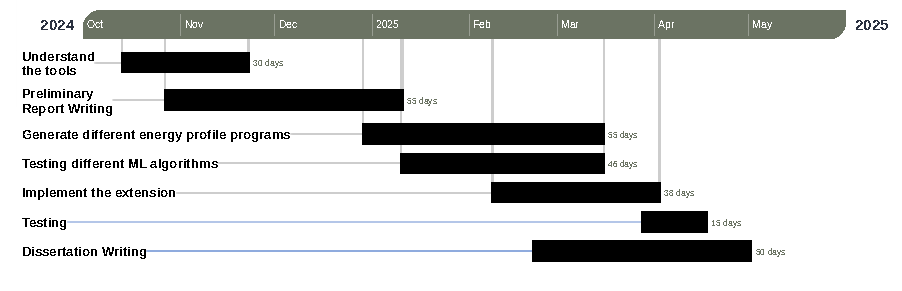
\includegraphics[width = 1 \textwidth]{figures/gantt_diagram.pdf}
%  \caption{Work Plan}
%  \label{fig:gantt_diagram}
%\end{figure*}


%The work plan is illustrated more clearly in Figure \ref{fig:gantt_diagram}, which provides a visual representation of the described tasks. While the dates shown in the figure may not precisely align with the actual timeline, the sequence of tasks remains accurate.